\chapter {Release 2 : Intégration d'IA et analyse des données}

\section{Introduction}
Dans ce quatrième chapitre, nous détaillerons le déroulement de la deuxième Release. Nous débuterons par la présentation des backlogs du troisème et qutarième sprints, accompagnée des diagrammes de classes
correspondants. Ensuite, nous exposerons les diagrammes de cas d’utilisation illustrant les différentes
fonctionnalités, ainsi que les diagrammes de séquence pour certaines tâches spécifiques liées à cette
release. \\
Enfin, nous concluons en présentant quelques interfaces démontrant les fonctionnalités implémentées.

\section{Sprint 3}
\subsection{Objectifs du sprint 3}
L’objectif de ce sprint est de permettre aux utilisateurs d’interagir directement avec le chatbot IA, en s’assurant qu’ils obtiennent des réponses pertinentes à leurs demandes. Il vise également à mettre en place une interface conviviale et intuitive, afin de rendre l’expérience d’utilisation simple et agréable.
\subsection{Backlog Sprint 3}

\begin{table}[H]
\centering
\renewcommand{\arraystretch}{1.4}
\resizebox{\textwidth}{!}{%
\begin{tabular}{|
>{\centering\arraybackslash}m{1cm}|
>{\centering\arraybackslash}m{4cm}|
>{\centering\arraybackslash}m{1cm}|
m{6cm}|
>{\centering\arraybackslash}m{2cm}|
>{\centering\arraybackslash}m{2cm}|
>{\centering\arraybackslash}m{2cm}|}
\hline
\textbf{ID} & \textbf{Module} & \textbf{Story ID} & \textbf{User Story} & \textbf{Priorité} & \textbf{Complexité} & \textbf{Nb jours} \\
\hline

\multirow{4}{*}{3} & \multirow{4}{4cm}{Intégration Model IA}  
& 3.1 & En tant qu’utilisateur, je veux discuter avec le chatbot IA & Élevé & L & 12 \\
\cline{3-7}
& & 3.2 & En tant qu’utilisateur, je veux recevoir des réponses pertinentes du chatbot & Élevé & M & 4 \\
\cline{3-7}
& & 3.3 & En tant qu’utilisateur, je veux une interface conviviale pour interagir avec l’IA & Moyen & M & 4 \\
\cline{3-7}
& & 3.4 & En tant qu’administrateur, je veux consulter mon historique du chat & Faible & S & 2 \\
\hline

\end{tabular}%
}
\captionsetup{justification=centering}
\caption{Backlog Sprint 3}
\label{tab:BacklogSprint3}
\end{table}

Le tableau 4.1 représente le backlog du sprint 3.

\subsection{Etude conceptuelle du sprint 3}
\subsubsection{Use case du sprint 3}
La figure 4.1 représente le diagramme de cas d'utilisation du sprint 3
\begin{figure}[H]
    \centering
    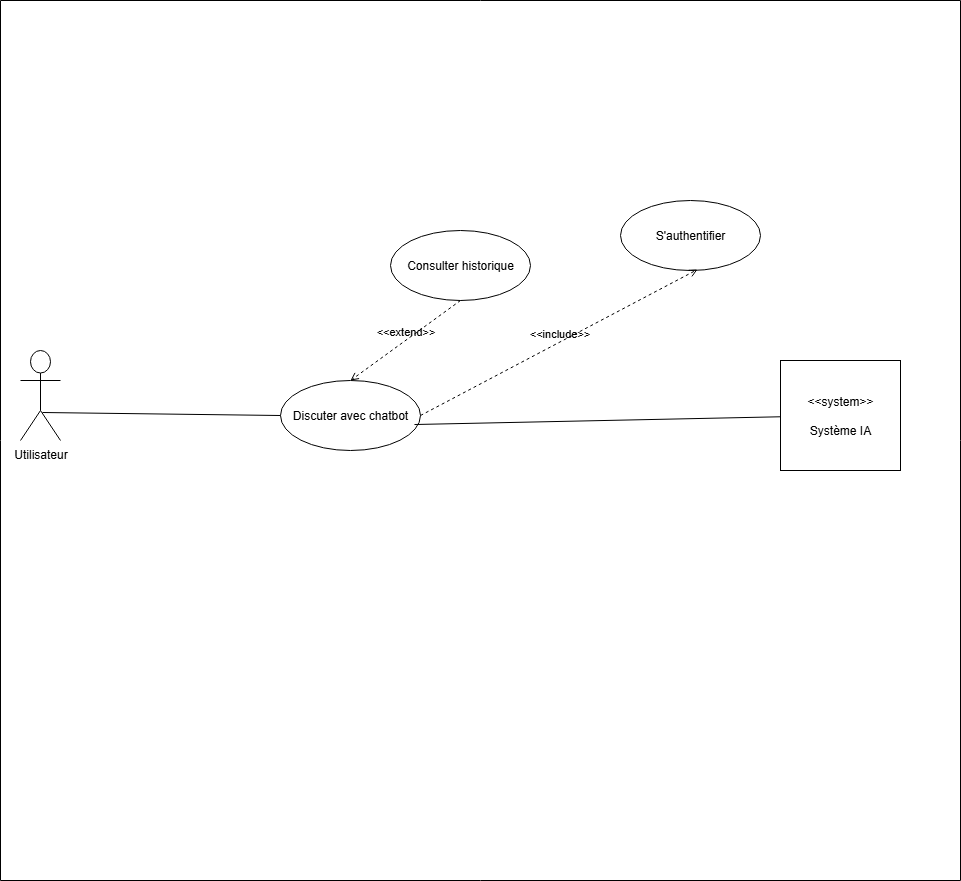
\includegraphics[width=1\linewidth]{img/sprint3usecasefv.png}
    \caption{Diagramme de cas d'utilisation du sprint 3}
    \label{fig:enter-label}
\end{figure}
\subsubsection{Diagramme de classes sprint 3}
Cette figure 4.2 réppresente le diagramme de classes du troisème sprint :

\begin{figure}[H]
    \centering
    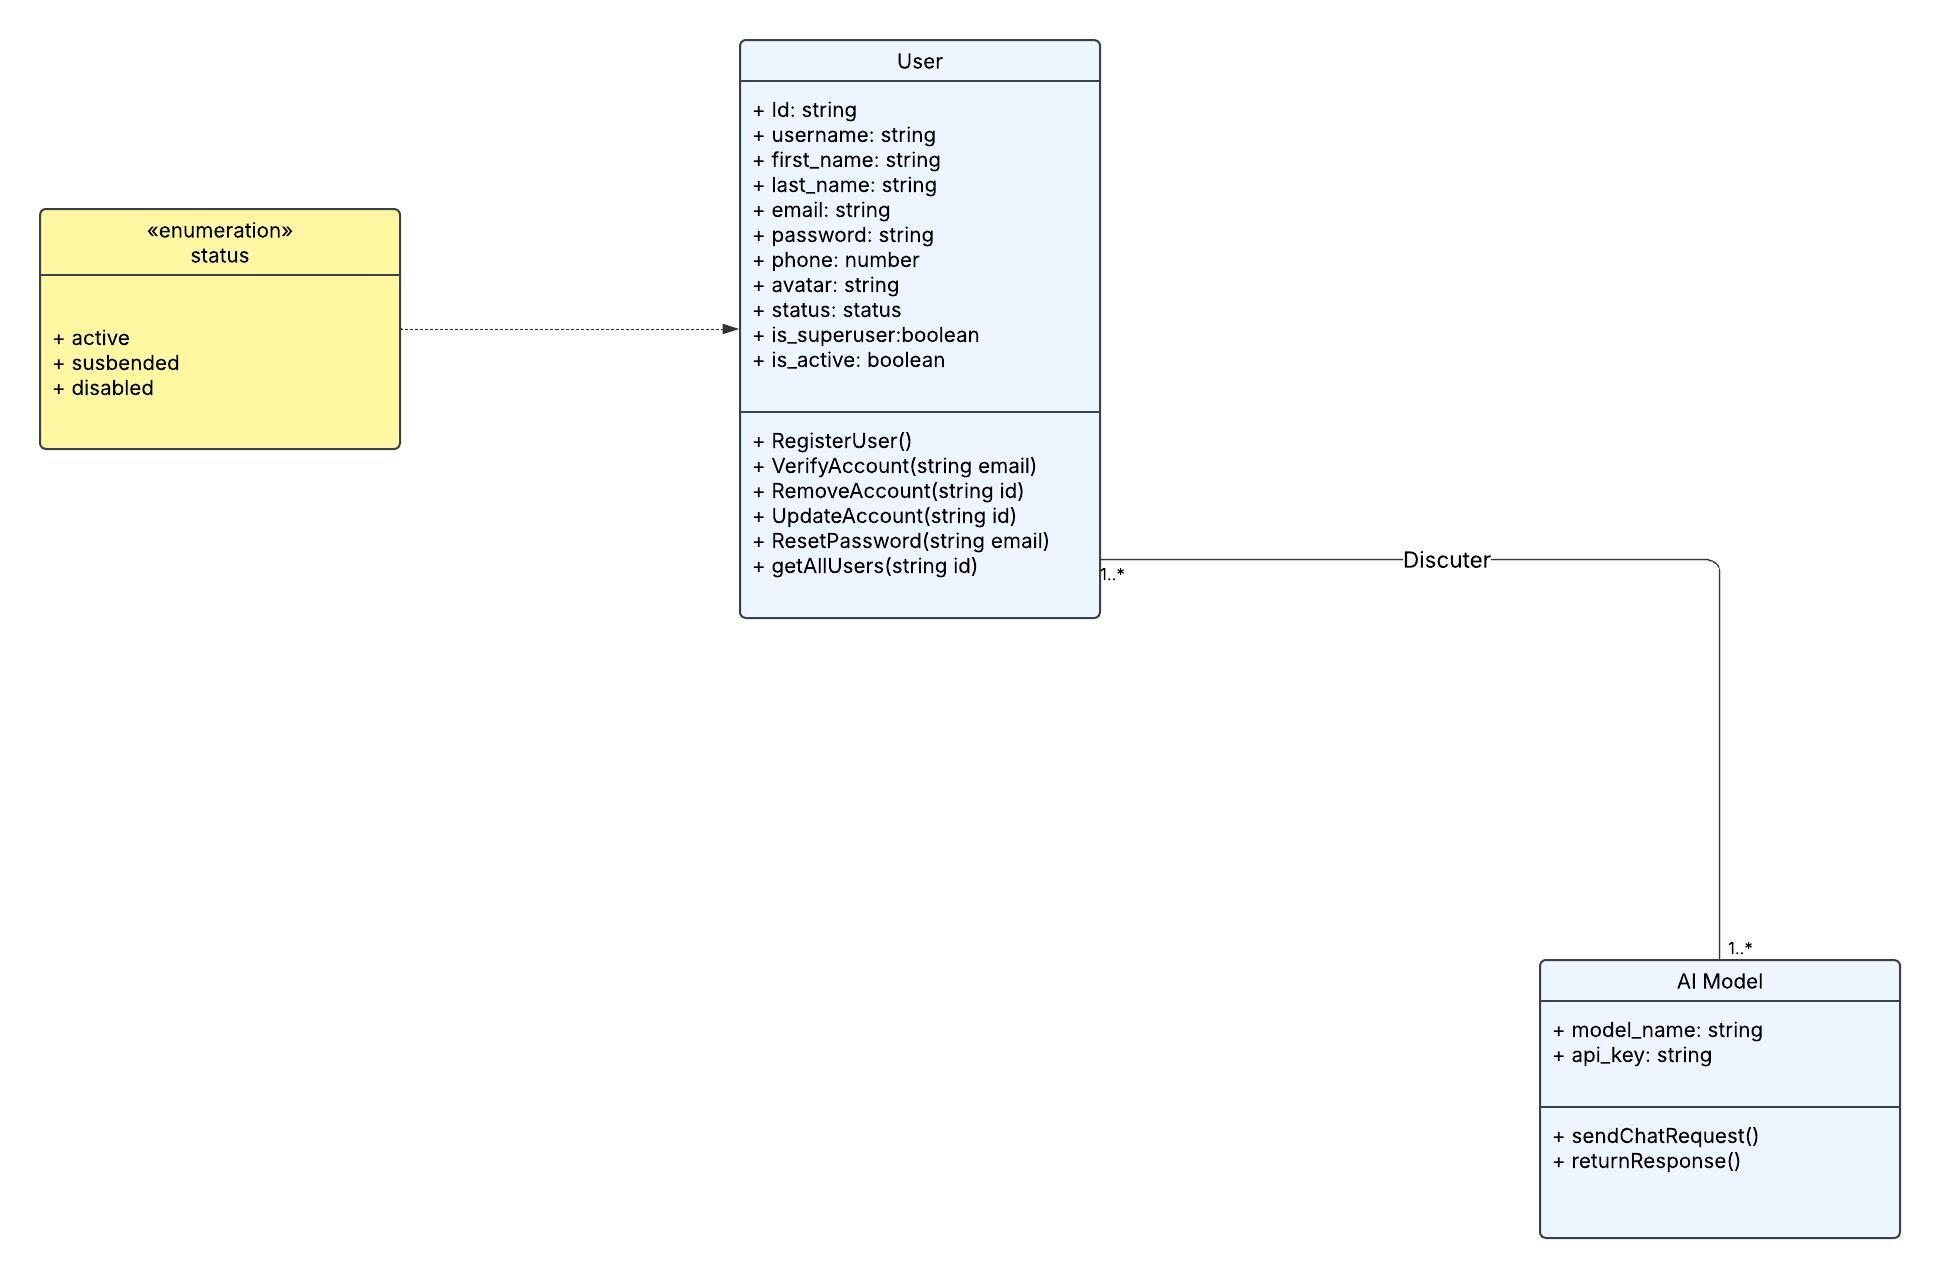
\includegraphics[width=1.15\linewidth]{img/Sprint3ClassesDiagram.jpeg}
    \caption{Diagramme de classes Sprint 3}
    \label{fig:enter-label}
\end{figure}

\subsection{ Descriptions des cas d’utilisation}




\begin{itemize} [label=\textbullet]
    \item \textbf{Description textuelle du cas d’utilisation discuter avec le chatbot}
\end{itemize} 
Le tableau 4.2 représnte la description textuelle du cas d'utilisation discuter avec chatbot
\begin{longtable}{|>{\raggedright\arraybackslash}p{4cm}|>{\raggedright\arraybackslash}p{11cm}|}
\hline
\textbf{Cas d’utilisation} & discuter avec le chatbot \\
\hline
\textbf{Acteur(s)} & Utilisateur \\
\hline
\textbf{Pré-condition} & L'utilisateur doit être authentifié . \\
\hline
\textbf{Post-condition} & Session du chat créer \\
\hline
\textbf{Scénario nominal} &
1.L'utilisateur visite la page permettant de discuter avec l'IA. . \newline
2. L'utilisateur tape un prompt. . \newline
3. Le modèle d'IA répond à ce prompt \newline
4. L'utilisateur poursuit la discussion . \\
\hline
\textbf{Scénario alternatif} &
- Erreur de connexion avec le modéle IA . \newline
- Le prompt a dépassé le nombre maximal de tokens autorisés. \\
\hline


\captionsetup{justification=centering}
\caption{Description textuelle du cas d’utilisation "discuter avec le chatbot"}
\label{tab:Description textuelle du cas d’utilisation "discuter avec le chatbot"s}
\end{longtable}

\begin{itemize} [label=\textbullet]
    \item \textbf{Diagramme de séquence "discuter avec le chatbot"}
\end{itemize} 

La figure 4.3 représente le diagramme de séquence discuter avec chatbot

\begin{figure}[H]
    \centering
    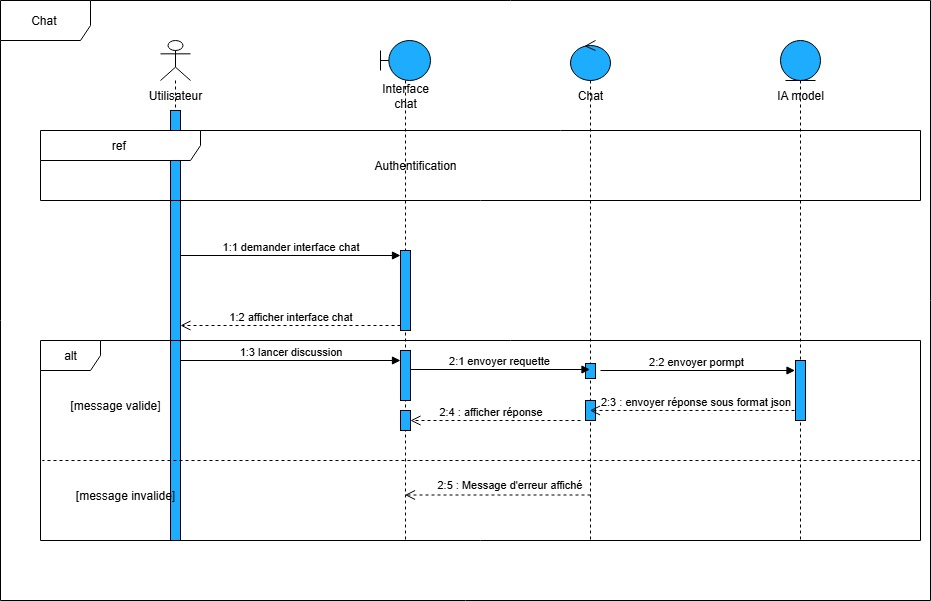
\includegraphics[width=1\linewidth]{img/iadiscussseqdiagfinalversion.jpg}
    \caption{Diagramme de séquence "discuter avec le chatbot"}
    \label{fig:enter-label}
\end{figure}

\subsection{Réalisation du Sprint 3} 


\begin{itemize} [label=\textbullet]

\item \textbf {Interfaces discuter avec chatbot :}


La figure 4.4 présente l'interface de chat 

\begin{figure}[H]
    \centering
    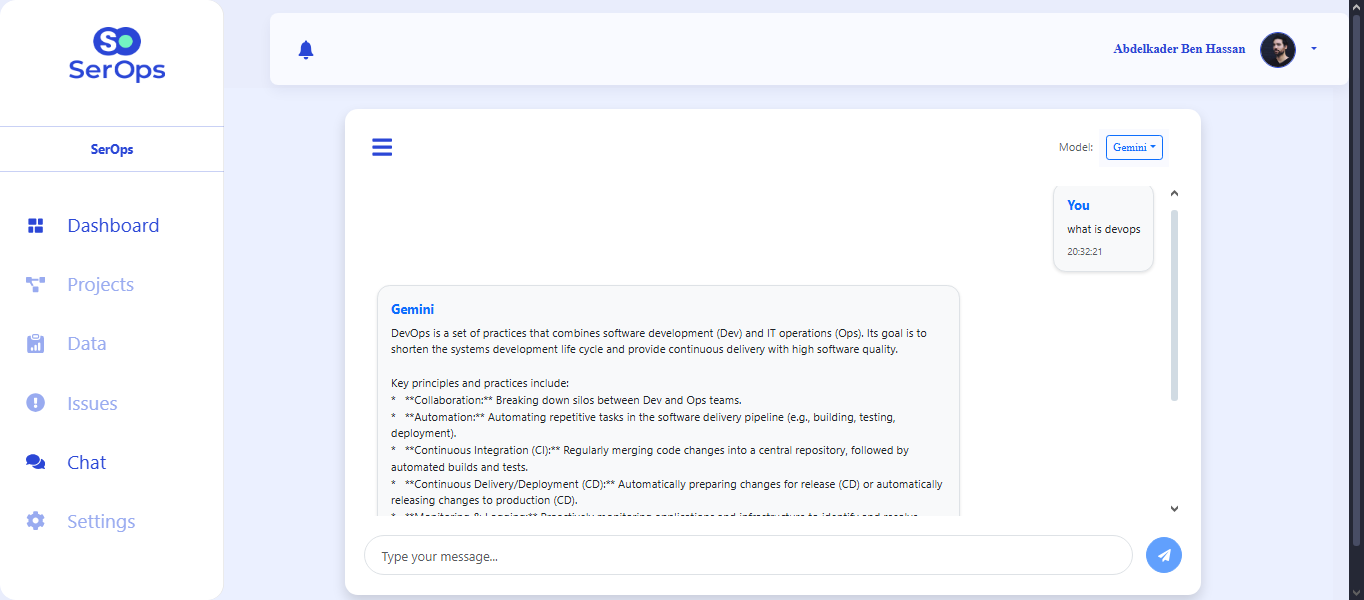
\includegraphics[width=1\linewidth]{img/ChatInterface.png}
    \caption{Interface Chat}
    \label{fig:enter-label}
\end{figure}

\clearpage


\item \textbf {Interface historique chat :}

la figure 4.5 présente l'historique et les sessions du chat dans laquelle l'utilisateur peut completer son discussion et consulter l'historique des chat

\begin{figure}[H]
    \centering
    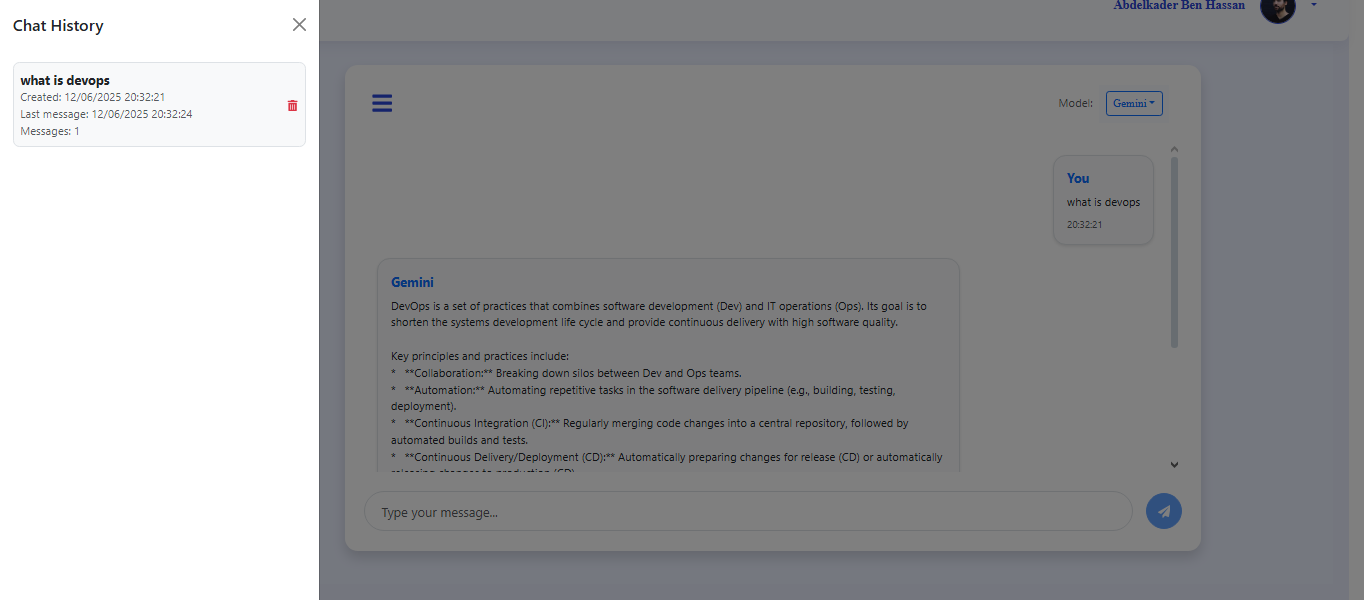
\includegraphics[width=1\linewidth]{img/ChatHistory.png}
    \caption{Interface Chat History}
    \label{fig:enter-label}
\end{figure}

\end{itemize}

\section{Sprint 4}
\subsection{Objectifs du sprint 4}
L’objectif de ce sprint est de mettre en place l’analyse des logs et des métriques afin de permettre aux utilisateurs de consulter les anomalies détectées par l’IA. Il vise également à offrir la possibilité d’accéder aux solutions proposées et d’interagir avec l’IA pour affiner les actions, tout en permettant la réanalyse des données avec le même ou un autre modèle d’IA.
\subsection{Backlog Sprint 4}

\begin{table}[H]
\centering
\renewcommand{\arraystretch}{1.4}
\resizebox{\textwidth}{!}{%
\begin{tabular}{|
>{\centering\arraybackslash}m{1cm}|
>{\centering\arraybackslash}m{4cm}|
>{\centering\arraybackslash}m{1cm}|
m{6cm}|
>{\centering\arraybackslash}m{2cm}|
>{\centering\arraybackslash}m{2cm}|
>{\centering\arraybackslash}m{2cm}|}
\hline
\textbf{ID} & \textbf{Module} & \textbf{Story ID} & \textbf{User Story} & \textbf{Priorité} & \textbf{Complexité} & \textbf{Nb jours} \\
\hline

\multirow{3}{*}{4} & \multirow{3}{4cm}{Analyse des logs et des métriques}  
& 4.1 & En tant qu’administrateur, je veux consulter les anomalies détectées par l'IA après l’analyse des données & Élevé & M & 10 \\
\cline{3-7}
& & 4.2 & En tant qu’administrateur, je veux accéder aux solutions proposées par l’IA et continuer la discussion pour évaluer ou affiner les actions & Élevé & L & 12 \\
\cline{3-7}
& & 4.3 & En tant qu’administrateur, je veux renvoyer les données afin de les analyser à nouveau avec un autre modèle d’IA ou pour les réanalyser & Élevé & M & 8 \\
\hline

\end{tabular}%
}
\captionsetup{justification=centering}
\caption{Backlog Sprint 4}
\label{tab:BacklogSprint4}
\end{table}

Le tableau 4.3 représente le backlog du sprint 4.

\subsection{Etude conceptuelle du sprint 4}
\subsubsection{Use Case sprint 4}
La figure 4.6 resprésente le diagramme de cas d'utilisation du sprint 4 
\begin{figure}[H]
    \centering
    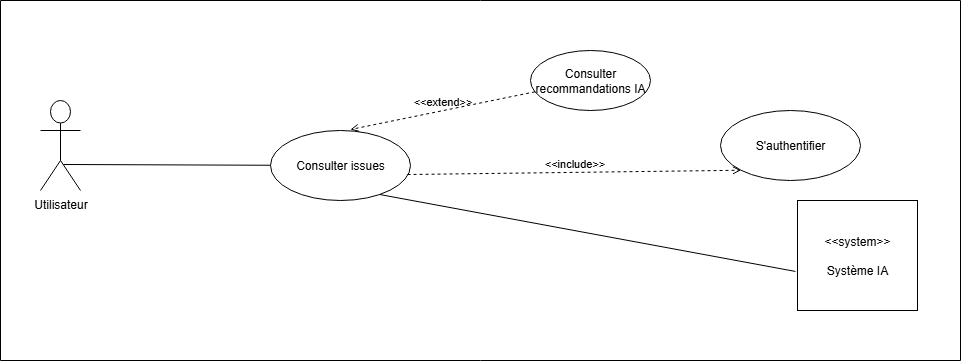
\includegraphics[width=1\linewidth]{img/Sprint4USeCase.png}
    \caption{Diagramme de cas d'utilisation du Sprint 4}
    \label{fig:enter-label}
\end{figure}
\subsubsection{Diagramme de classes sprint 4}
Cette figure 4.7 réppresente le diagramme de classes du sprint 4:


\begin{figure}[H]
    \centering
    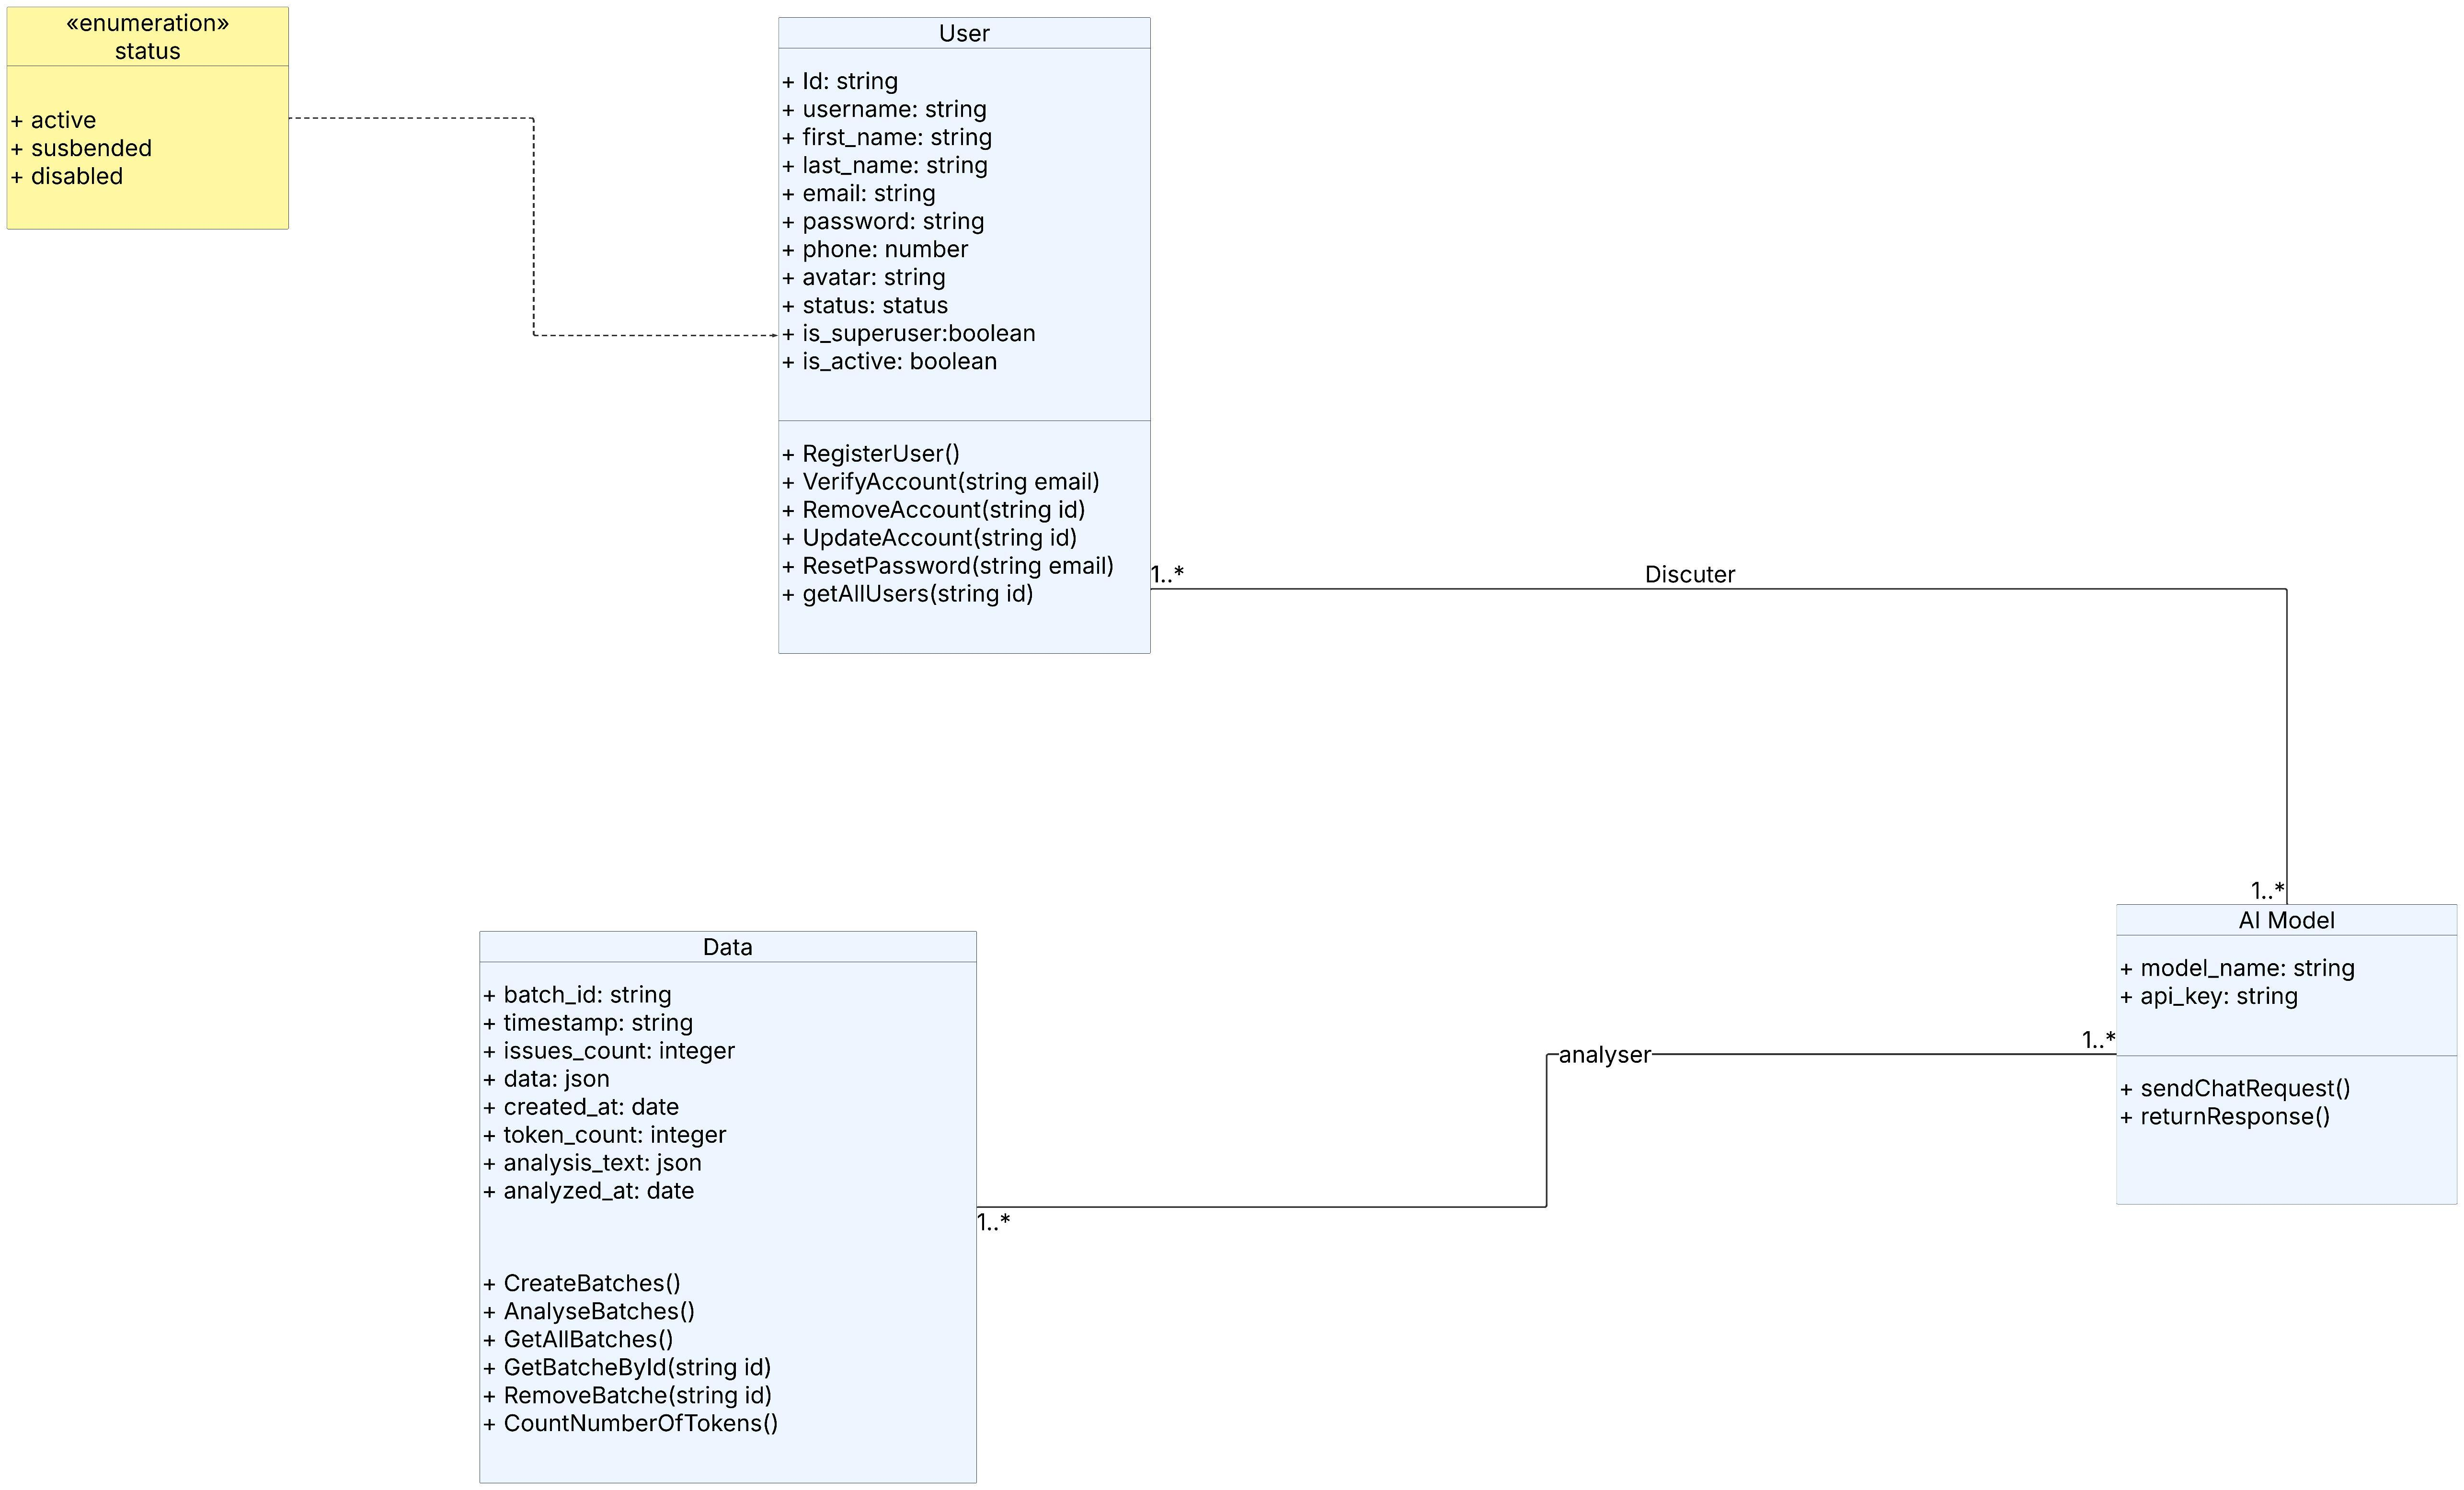
\includegraphics[width=1.15\linewidth]{img/Sprint4ClassesFV.jpeg}
    \caption{Diagramme de classes Sprint 4}
    \label{fig:enter-label}
\end{figure}

\subsubsection{ Descriptions textuelle des cas d’utilisation}

Le tableau 4.4 représente la description textuelle du cas d'utilisation consulter anomalies

\begin{itemize} [label=\textbullet]
    \item \textbf{Description textuelle du cas d’utilisation consulter anomalies}
\end{itemize} 
\begin{longtable}{|>{\raggedright\arraybackslash}p{4cm}|>{\raggedright\arraybackslash}p{11cm}|}
\hline
\textbf{Cas d’utilisation} & Consulter anomalies \\
\hline
\textbf{Acteur(s)} & Utilisateurs \\
\hline
\textbf{Pré-condition} & L'utilisateur doit être authentifié . \\
\hline
\textbf{Post-condition} & Anomalies Affiché \\
\hline
\textbf{Scénario nominal} &
1. L'utilisateur visite la page qui affiche les anomalies. \newline
2. L’utilisateur choisi une anomalies a consulter . \newline
3. Le système affiche la cause de cette anomalie et action recommandée pour résoudre ce problème . \newline \\
\hline
\textbf{Scénario alternatif} &
- Pas des anomalies disponible . \\
\hline


\captionsetup{justification=centering}
\caption{Description textuelle du cas d’utilisation consulter anomalies}
\label{tab:Description textuelle du cas d’utilisation consulter anomalies}
\end{longtable}

\begin{itemize} [label=\textbullet]
    \item \textbf{Diagramme de séquence "consulter anomalies"}
\end{itemize} 

La figure 4.8 représente le diagramme de cas d'utilisation consulter anomalie

\begin{figure}[H]
    \centering
    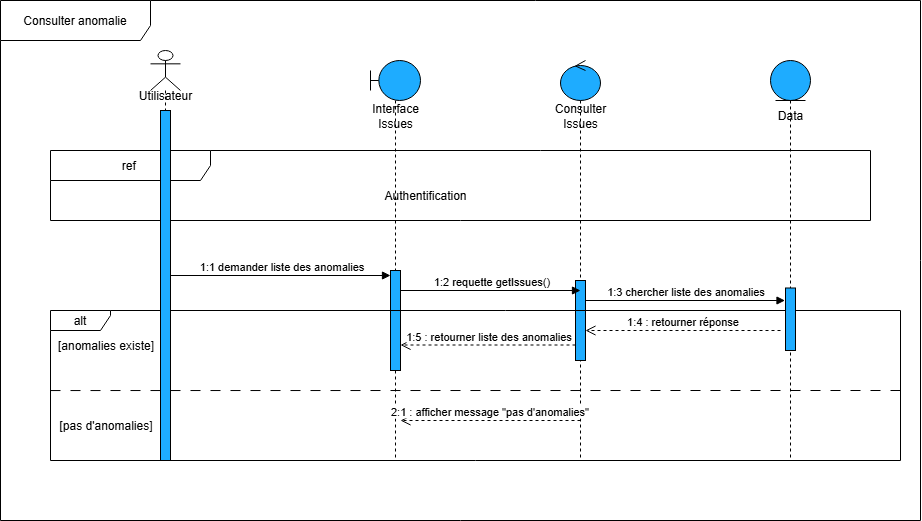
\includegraphics[width=1\linewidth]{img/issuesseqfv (1).png}
    \caption{Diagramme de cas d'utilisation consulter anomalie}
    \label{fig:enter-label}
\end{figure}





\begin{itemize} [label=\textbullet]
    \item \textbf{Description textuelle du cas d’utilisation  accéder aux solutions proposées par l’IA}
\end{itemize} 
Le tableau 4.5 représente la description textuelle du cas d'utilisation consulter solution IA

\begin{longtable}{|>{\raggedright\arraybackslash}p{4cm}|>{\raggedright\arraybackslash}p{11cm}|}
\hline
\textbf{Cas d’utilisation} & accéder aux solutions proposées par l’IA \\
\hline
\textbf{Acteur(s)} & Administrateur \\
\hline
\textbf{Pré-condition} & L'utilisateur doit être authentifié . \\
\hline
\textbf{Post-condition} & Solution IA Affiché \\
\hline
\textbf{Scénario nominal} &
1. L'utilisateur visite la page qui affiche les anomalies. \newline
2. L’utilisateur choisi la solution d'anomalie proposer par l'IA . \newline
3. Le système affiche la page du discussion de cette anomalie et l'action recommandée pour résoudre ce problème . \newline
\\

\hline
\textbf{Scénario alternatif} &
- Erreur de connexion au modéle IA . \newline
- Pas d'action pour résoudre l'anomalie.
\\
\hline


\captionsetup{justification=centering}
\caption{Description textuelle du cas d’utilisation consulter anomalies}
\label{tab:Description textuelle du cas d’utilisation consulter anomalies}
\end{longtable}



\begin{itemize} [label=\textbullet]
    \item \textbf{Diagramme de séquence "accéder aux solutions proposées par l’IA"}
\end{itemize} 

La figure 4.9 représente le diagramme de séquence accéder aux solutions proposées par l’IA

\begin{figure}[H]
    \centering
    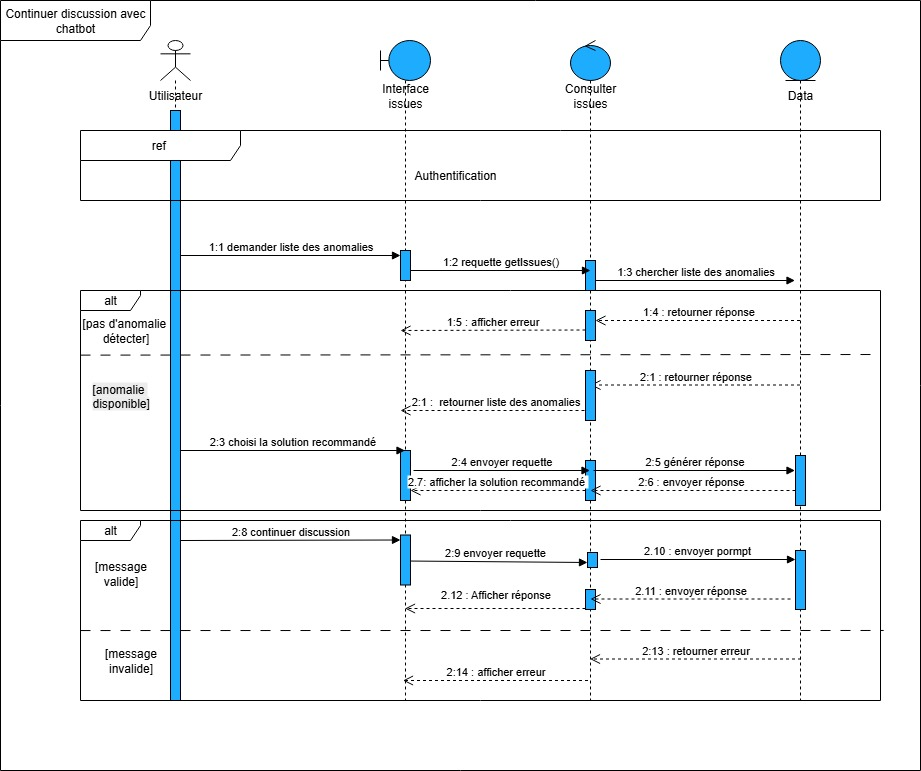
\includegraphics[width=1\linewidth]{img/completechat (1) (2).jpg}
    \caption{Digramme de séquence accéder aux solutions proposées par l’IA}
    \label{fig:enter-label}
\end{figure}



\subsubsection{Analyser à nouveau les data.}




\begin{itemize} [label=\textbullet]
    \item \textbf{Description textuelle du cas d’utilisation analyser à nouveau les data}
\end{itemize} 
Le tableau 4.6 représente la description textuelle de cas d'utilisation consulter anomalies
\begin{longtable}{|>{\raggedright\arraybackslash}p{4cm}|>{\raggedright\arraybackslash}p{11cm}|}
\hline
\textbf{Cas d’utilisation} & analyser à nouveau les data \\
\hline
\textbf{Acteur(s)} & Administrateur \\
\hline
\textbf{Pré-condition} & L'utilisateur doit être authentifié . \\
\hline
\textbf{Post-condition} & Anomalies Affiché \\
\hline
\textbf{Scénario nominal} &
1. L'utilisateur visite la page qui affiche les data. \newline
2. L’utilisateur choisi une ou plusieurs data a analyser . \newline
3. l'utilisateur choisi le modèle IA . \newline
4. Le système affiche l'interface de chat contient le resultat d'analyse de cette anomalie et action recommandée pour résoudre ce problème . \newline
5. L'utilisateur continuer la discussion .
\\
\hline
\textbf{Scénario alternatif} &
- Erreur de connexion au modéle IA . \newline
- Pas Data disponible . \newline 
\\
\hline


\captionsetup{justification=centering}
\caption{Description textuelle du cas d’utilisation consulter anomalies}
\label{tab:Description textuelle du cas d’utilisation consulter anomalies}
\end{longtable}


\begin{itemize} [label=\textbullet]
    \item \textbf{Diagramme d'état transition analyser data}
\end{itemize} 
La figure 4.10 représente le diagramme d'état transition analyser data

\begin{figure}[H]
    \centering
    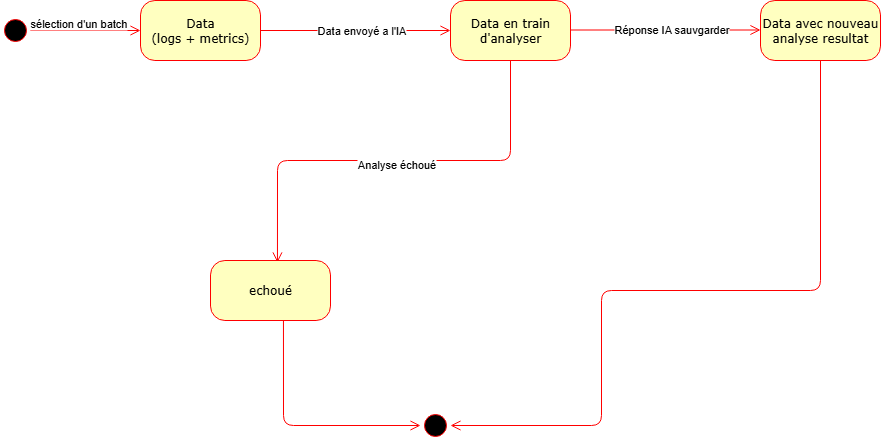
\includegraphics[width=1\linewidth]{img/statediagramme.png}
    \caption{Digramme état transition}
    \label{fig:enter-label}
\end{figure}

\subsection{Réalisation du Sprint 4}

Dans cette section nous allons présenter les interface réalisées pour Sprint 4


\begin{itemize} [label=\textbullet]

\item \textbf {Interface anomalies :}

La figure 4.11 présente la liste des  anomalies détecter dans les batches par l'IA

\begin{figure}[H]
    \centering
    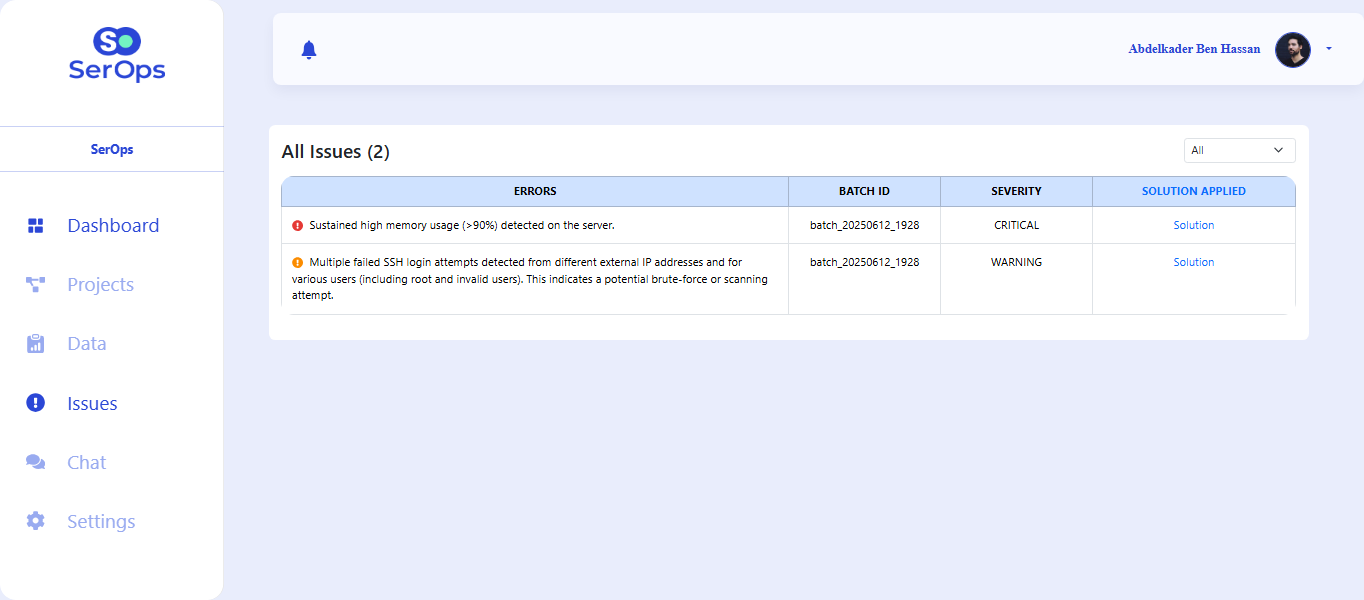
\includegraphics[width=1\linewidth]{img/IssuesPage.png}
    \caption{Interface Issues}
    \label{fig:enter-label}
\end{figure}

\item \textbf{Interface action recommandé par l'IA}

La figure 4.12 représente l'interface action recommandé par l'IA

\begin{figure}[H]
    \centering
    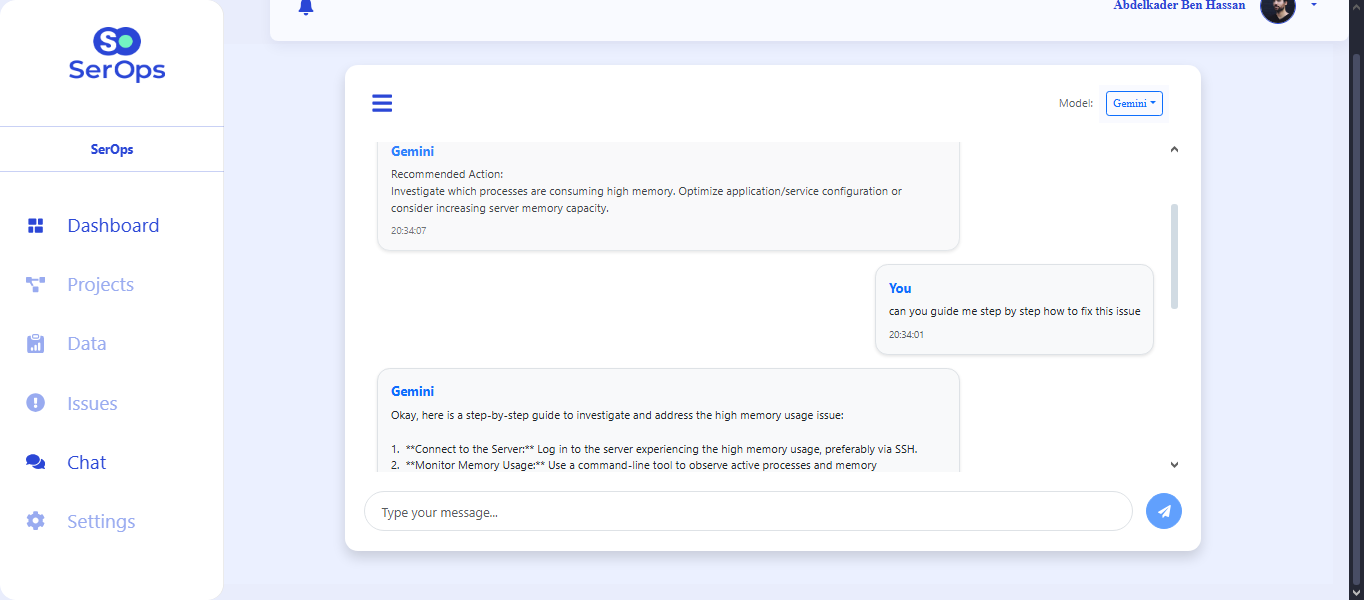
\includegraphics[width=1\linewidth]{img/RecommandedActions.png}
    \caption{Interface Recommanded actions}
    \label{fig:enter-label}
\end{figure}


\item \textbf {Interface refaire l'analyse :}

La figure 4.13 interface l'utilisateur peux se analyser à nouveau les data et choisir le modèle IA  :

\begin{figure}[H]
    \centering
    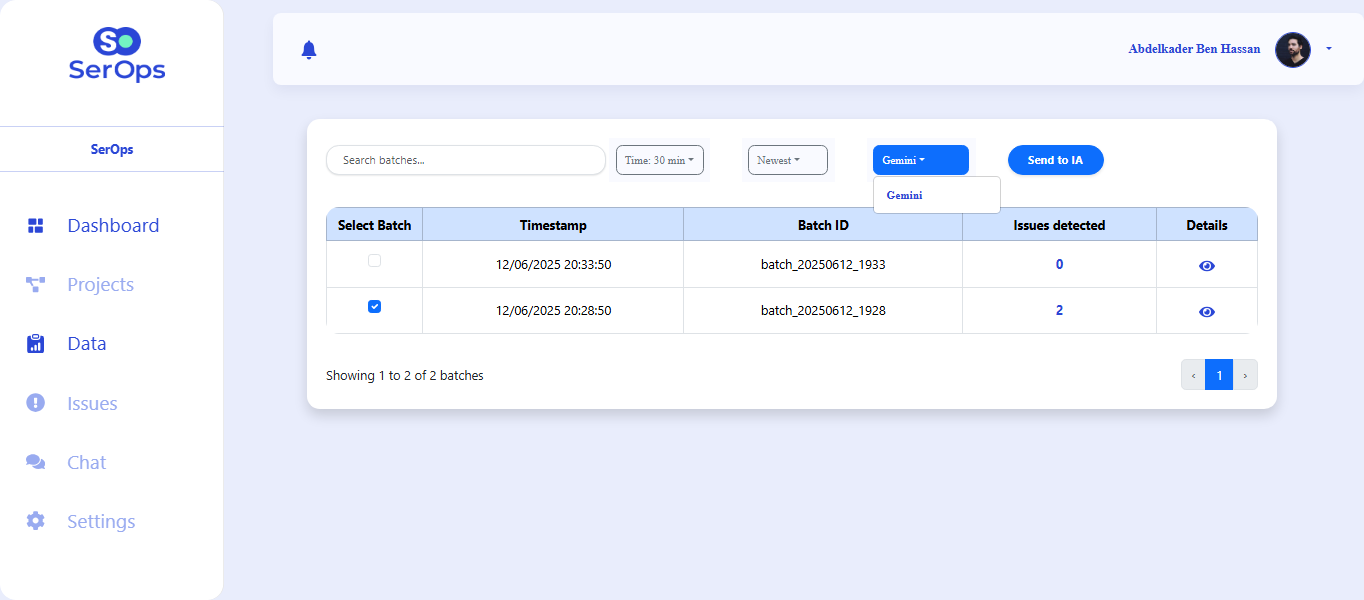
\includegraphics[width=1\linewidth]{img/Reanalyser.png}
    \caption{Interface analyser data}
    \label{fig:enter-label}
\end{figure}
\end{itemize}

\section{Conclusion}
Dans ce chapitre, nous avons détaillé les user stories correspondant aux troisième et quatrième sprints. Par la suite, nous avons présenté la conception mise en place durant cette phase. Enfin, nous avons exposé les éléments liés à la réalisation de la seconde moitié de notre application, en illustrant notre propos à l’aide de captures d’écran des différentes interfaces développées.

Dans le chapitre suivant, nous aborderons la troisième release de notre application, centrée sur la gestion des projets et des utilisateurs, intégrant notamment l’analyse automatisée des logs CI/CD ainsi que la gestion des rôles et des états des utilisateurs.
